\documentclass[10pt,landscape]{article}
\usepackage{multicol}
\usepackage{calc}
\usepackage{ifthen}
\usepackage[landscape]{geometry}
\usepackage{hyperref}
\usepackage{graphicx}
\usepackage{amsmath}
\usepackage{tikz}
\usetikzlibrary{shapes.geometric, arrows, calc, positioning}
\usepackage[table]{xcolor}
\usepackage{tabularx}
\usepackage{booktabs}
\usepackage{float}
\usepackage{amssymb}

\ifthenelse{\lengthtest { \paperwidth = 11in}}
    { \geometry{top=.5in,left=.5in,right=.5in,bottom=.5in} }
    {\ifthenelse{ \lengthtest{ \paperwidth = 297mm}}
        {\geometry{top=1cm,left=1cm,right=1cm,bottom=1cm} }
        {\geometry{top=1cm,left=1cm,right=1cm,bottom=1cm} }
    }

\pagestyle{empty}

\makeatletter
\renewcommand{\section}{\@startsection{section}{1}{0mm}%
                                {-1ex plus -.5ex minus -.2ex}%
                                {0.5ex plus .2ex}%
                                {\normalfont\large\bfseries}}
\renewcommand{\subsection}{\@startsection{subsection}{2}{0mm}%
                                {-1ex plus -.5ex minus -.2ex}%
                                {0.5ex plus .2ex}%
                                {\normalfont\normalsize\bfseries}}
\renewcommand{\subsubsection}{\@startsection{subsubsection}{3}{0mm}%
                                {-1ex plus -.5ex minus -.2ex}%
                                {1ex plus .2ex}%
                                {\normalfont\small\bfseries}}
\makeatother

\setlength{\parindent}{0pt}
\setlength{\parskip}{0pt plus 0.5ex}

\begin{document}
\begin{multicols}{3}

% ─────────────────────────────────────────
\section{Congestion Control}
% ─────────────────────────────────────────

\textbf{Key terms:} Link Capacity $R$, Congestion Window \texttt{cwnd}, $N$ Hosts\\
Ideal throughput: $R/N$ \quad Measured: $\frac{\text{\#bytes in RTT}}{RTT}$

\textbf{Cost of Congestion:}
\begin{itemize}\setlength\itemsep{0pt}
  \item Retransmissions (packet lost)
  \item Unneeded retransmits (full buffer $\Rightarrow$ 2x send)
  \item Buffering wasted for packets lost downstream
\end{itemize}

\textbf{Types:} Loss-based (TCP Reno/Cubic) $|$ Delay-based (Vegas) $|$ ECN (L4S)

TCP uses a \textbf{sliding window} via \texttt{cwnd}.\\
\textbf{TCP Reno:} 3 dup ACK $\rightarrow$ SR $= \tfrac{1}{2}$\\
\textbf{TCP Tahoe:} timeout $\rightarrow$ SR $= 1$ MSS\\
\textbf{Slow-start:} cwnd $= 1$, double per round (cwnd++ per ACK); switch to linear after loss; threshold = pre-loss cwnd.

\resizebox{\columnwidth}{!}{%
    \rotatebox{90}{%
        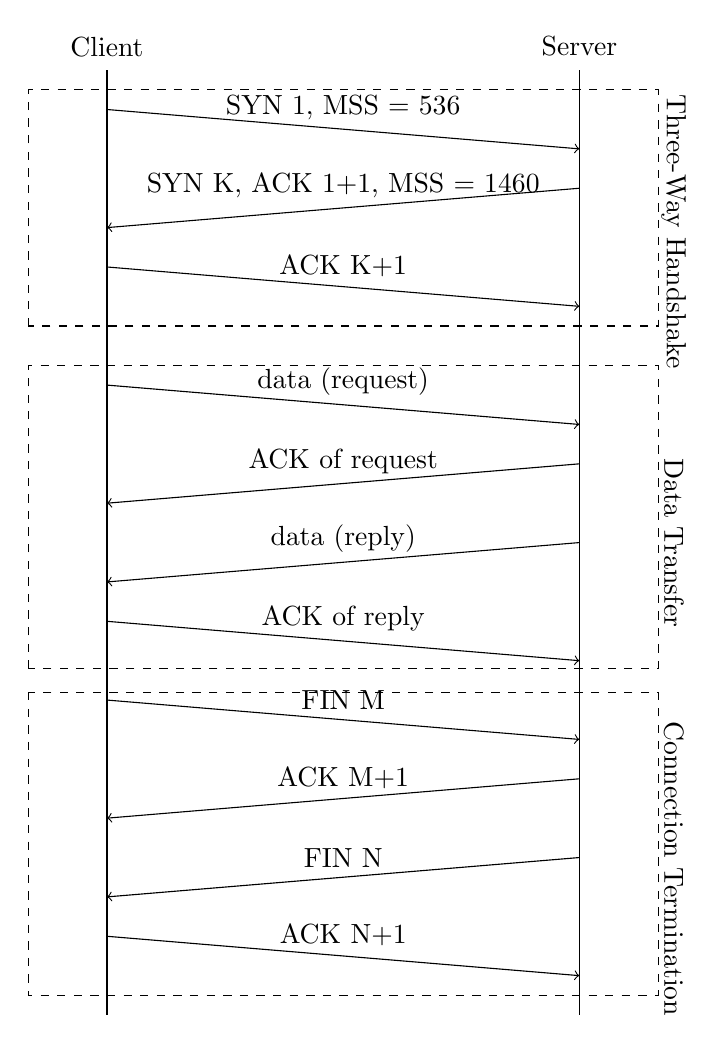
\begin{tikzpicture}
            % Drawing the vertical lines for Client and Server
            \draw (-3,0) -- (-3,-12) (3,0) -- (3,-12);
            
            % Labels for Client and Server
            \node at (-3,.3) {Client};
            \node at (3,.3) {Server};
            
            % Three-Way Handshake
            \draw[->] (-3,-0.5) -- node[midway,above] {SYN 1, MSS = 536} (3,-1);
            \draw[->] (3,-1.5) -- node[midway,above] {SYN K, ACK 1+1, MSS = 1460} (-3,-2);
            \draw[->] (-3,-2.5) -- node[midway,above] {ACK K+1} (3,-3);
            
            % Data Exchange
            \draw[->] (-3,-4) -- node[midway,above] {data (request)} (3,-4.5);
            \draw[->] (3,-5) -- node[midway,above] {ACK of request} (-3,-5.5);
            \draw[->] (3,-6) -- node[midway,above] {data (reply)} (-3,-6.5);
            \draw[->] (-3,-7) -- node[midway,above] {ACK of reply} (3,-7.5);
            
            % Connection Termination
            \draw[->] (-3,-8) -- node[midway,above] {FIN M} (3,-8.5);
            \draw[->] (3,-9) -- node[midway,above] {ACK M+1} (-3,-9.5);
            \draw[->] (3,-10) -- node[midway,above] {FIN N} (-3,-10.5);
            \draw[->] (-3,-11) -- node[midway,above] {ACK N+1} (3,-11.5);
            \draw[dashed] (-4,-3.25) rectangle (4,-0.25) 
            node[rotate=270, anchor=west, yshift=0.2cm, xshift=-2] {Three-Way Handshake};
        
            \draw[dashed] (-4,-7.6) rectangle (4,-3.75) 
            node[rotate=270, anchor=west, yshift=0.2cm, xshift=30] {Data Transfer};
        
            \draw[dashed] (-4,-7.9) rectangle (4,-11.75) 
            node[rotate=270, anchor=west, yshift=0.2cm, xshift=-102.5] {Connection Termination};
        \end{tikzpicture}
    }
}

\textbf{ECN:} Sender sets ECN bits (01) in IP header; router marks 11 on congestion; receiver sets ECE bit in ACK.

\textbf{L4S} (Low Latency, Low Loss, Scalable — IPv4+IPv6):
\begin{itemize}\setlength\itemsep{0pt}
  \item No drops, only marks $\rightarrow$ congestion signaling
  \item No starvation; coexists with non-L4S traffic
  \item Prioritizes L4S; goals: max throughput, min latency
  \item Prague theorem
  \item Datarate: $r = \frac{1}{p}-1$ [Mbps], $p$ = packet marking prob.
\end{itemize}

\textbf{Fairness:} $R/N$ \quad UDP: constant rate, no CC \quad TCP: allows parallel connections.

% ─────────────────────────────────────────
\section{Flow Control}
% ─────────────────────────────────────────

\textbf{Goal:} Don't overflow receiver buffer.\\
Link Capacity $R$: physical interface bandwidth of interconnect cable.\\
\textbf{Window-based FC:} Max data allowed without ACK (packet loss).\\
\textbf{Rate-based FC:} Congestion window / sliding window TCP; rate chosen at start.

More speed: Use different algos from CC/FC:\\
$\rightarrow$ Loss-based vs.\ Delay-based vs.\ Hybrid/ECN\\
\textit{``If you can't make the pipe bigger, make the flow smarter''}
\begin{itemize}\setlength\itemsep{0pt}
  \item Multipath / Load Balancing
  \item Active Queue Management
  \item Traffic Compression $\rightarrow$ Better
\end{itemize}

% ─────────────────────────────────────────
\section{Buffering}
% ─────────────────────────────────────────

$n$ TCP flows $\Rightarrow$ $B = \dfrac{RTT \cdot C}{\sqrt{n}}$, \quad $C$ = Capacity

% ─────────────────────────────────────────
\section{Congestion vs Flow Control}
% ─────────────────────────────────────────

Congestion $\approx$ too many senders $\neq$ Flow Control $\approx$ one sender too fast.\\
$\Rightarrow$ Long delays, queueing, packet loss, overflow.

% ─────────────────────────────────────────
\section{Packet Classification}
% ─────────────────────────────────────────

\textbf{Why:} Faster routes $|$ Allow good traffic $|$ Drop malicious

\textbf{Goals:}
\begin{itemize}\setlength\itemsep{0pt}
  \item Routing decision $\rightarrow$ select interface / fastest route
  \item Packet filtering $\rightarrow$ drop / allow
  \item Accounting $\rightarrow$ measure data
  \item Rate limiting
\end{itemize}

\subsection{Binary Representation IPv4}
\begin{center}
\textbf{12.4.0.0/15} \quad Mask: 255.254.0.0\\[2pt]
\begin{tabular}{r|c|c|c|c|}
Addr & \texttt{00001100} & \texttt{00000100} & \texttt{00000000} & \texttt{00000000}\\
Mask & \texttt{11111111} & \texttt{11111110} & \texttt{00000000} & \texttt{00000000}\\
\end{tabular}\\[2pt]
$\underbrace{\hspace{2.8cm}}_{\text{Network Prefix}}$ $\underbrace{\hspace{2.0cm}}_{\text{Hosts}}$
\end{center}

\subsection{Unibit Tries}

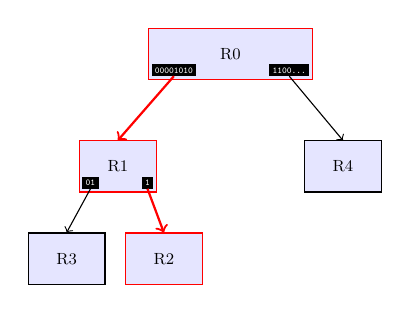
\begin{tikzpicture}[
    scale=0.65, transform shape,
    regnode/.style={draw, fill=blue!10, minimum width=3.2cm, minimum height=1cm, align=center, font=\small},
    smallreg/.style={draw, fill=blue!10, minimum width=1.5cm, minimum height=1cm, align=center, font=\small},
    bitbox/.style={draw, fill=black, text=white, font=\ttfamily\tiny, inner sep=1.5pt}
]
\node[regnode, draw=red] (R0) at (0,0) {R0};
\node[bitbox, anchor=south west] (R0L) at ($(R0.south west)+(2pt,2pt)$) {00001010};
\node[bitbox, anchor=south east] (R0R) at ($(R0.south east)+(-2pt,2pt)$) {1100...};

\node[smallreg, draw=red] (R1) at (-2.2,-2.2) {R1};
\node[bitbox, anchor=south west] (R1L) at ($(R1.south west)+(2pt,2pt)$) {01};
\node[bitbox, anchor=south east] (R1R) at ($(R1.south east)+(-2pt,2pt)$) {1};

\node[smallreg] (R4) at (2.2,-2.2) {R4};
\node[smallreg] (R3) at (-3.2,-4) {R3};
\node[smallreg, draw=red] (R2) at (-1.3,-4) {R2};

\draw[->,thick,draw=red] (R0L.south) -- (R1.north);
\draw[->] (R0R.south) -- (R4.north);
\draw[->] (R1L.south) -- (R3.north);
\draw[->,thick,draw=red] (R1R.south) -- (R2.north);
\end{tikzpicture}

Route P1: \texttt{10.128.12.1} $= \textcolor{red}{00001010.1}\ldots \rightarrow$ R2

\textbf{W-bit prefixes, N prefixes:} $\mathcal{O}(W)$ lookup, $\mathcal{O}(NW)$ storage, $\mathcal{O}(W)$ updates.

\subsection{Bit-Vector Linear Search}

Match ruleset: AND bit-vectors per field, pick highest-priority match.

\textbf{Scenario:} Packet \texttt{<123.25.1.1, 124, 123.25.4.0, 53, TCP>}

\begin{center}
{\footnotesize
\begin{tabular}{lccccccccc}
\toprule
\textbf{Field} & R1&R2&R3&R4&R5&R6&R7&R8\\
\midrule
Src-IP   & 1&1&1&1&0&1&1&1\\
Src-Port & 1&1&1&1&0&1&1&1\\
Dst-IP   & 1&1&0&1&0&1&1&1\\
Dst-Port & 0&1&1&0&0&1&1&1\\
Protocol & 1&0&1&1&0&1&1&1\\
\midrule
\textbf{AND} & 0&0&0&0&0&\textbf{1}&\textbf{1}&\textbf{1}\\
\bottomrule
\end{tabular}
}
\end{center}

Hits: R6, R7, R8 $\Rightarrow$ \textbf{Rule 6} (highest priority).\\
Complexity: $O(N \cdot d)$ time \& space; with word width $W$: $O(N/W)$ per field.

% ─────────────────────────────────────────
\section{IPv4 \& IPv6}
% ─────────────────────────────────────────

IPv4: 32-bit ($10^9$) \quad IPv6: 128-bit ($10^{38}$)\\
Interface: connects to link (virtual/physical)\\
\textbf{Netmask:} boundary between network \& host part\\
\textbf{Subnet border:} from interface, over links, to all connected interfaces

\textbf{Router:} connects networks $\Rightarrow$ VLAN/subnet traversal\\
\textbf{Switch:} connects devices in same network ($\rightarrow$ no L3, no IP)

\textbf{NAT:} One IP for all devices in a network\\
NAT Table: Ext.\ Address $|$ Ext.\ Interface $|$ Int.\ Address $|$ Int.\ Port\\
NAT: rewrite IP source $\rightarrow$ Layer 3, NAT Table in router.

IP Count: \#Interfaces $+ 2$ = Broadcast + Network Address

\textbf{Private IP Ranges:}\\
{\footnotesize
\begin{tabular}{ll}
0.0.0.0/8 & This network\\
10.0.0.0/8 & Local comms in priv. netw.\\
100.64.0.0/10 & Shared Carrier-Grade NAT\\
127.0.0.0/8 & Loopback\\
169.254.0.0/16 & Link-Local\\
172.16.0.0/12 & Local comms in priv. netw.\\
192.168.0.0/16 & Local comms in priv. netw.\\
224.0.0.0/4 & Multicast\\
\end{tabular}
}

Link Local Address = SLAAC (Stateless Address Autoconfiguration)

\textbf{IPv6 Special Addresses:}\\
{\footnotesize
\begin{tabular}{ll}
\texttt{::1/128} & Loopback\\
\texttt{::/128} & Unspecified\\
\texttt{::ffff:\textcolor{red}{X.X.X.X}/96} & IPv4 mapped\\
\texttt{64:ff9b::hex(X.X.X.X)/96} & NAT64\\
\texttt{5f00::/16} & IPv6 Segment Routing\\
\texttt{fc00::/7} & Unique Local Address\\
\texttt{fe80::/64} & Link Local Address\\
\texttt{ff00::/8} & Multicast Address\\
\texttt{2000::/3} & Global Unicast\\
\texttt{FC00::/7} & Unique Local Unicast\\
\texttt{fe80::/10} & Link-Local Unicast\\
\end{tabular}
}

% ─────────────────────────────────────────
\section{BGP}
% ─────────────────────────────────────────

AS $\leftrightarrow$ AS\\
\textbf{Intra:} Within same AS \quad \textbf{Inter:} Different AS\\
$\rightarrow$ Be careful who you choose (Cost, Privacy)\\
Tools: AS numbers in path\\
TCP Port 179\\
Messages: Open, Update, Keepalive, Notification

\textbf{Routing Information Protocol} $\rightarrow$ iBGP\\
Kürzeste Pfade in einem AS finden $\Rightarrow$ Hop Count

% ─────────────────────────────────────────
\section{Subnets}
% ─────────────────────────────────────────

Subnet = group of interfaces with same prefix.\\
/N mask $\Rightarrow$ $2^{32-N}$ host addresses (IPv4).\\
Always reserve: network addr.\ + broadcast addr.

% ─────────────────────────────────────────
\section{Collective Communication}
% ─────────────────────────────────────────

\textbf{Primitives:}
\begin{itemize}\setlength\itemsep{0pt}
  \item \textbf{Broadcast:} one node sends full vector $m$ to all
  \item \textbf{Scatter:} one node sends chunk $m/n$ to each node
  \item \textbf{Gather:} one node collects chunks from all $\rightarrow$ full vector
  \item \textbf{AllGather:} every node ends up with full vector (chunks from all)
  \item \textbf{Reduce:} one node collects \& applies op (sum/min/max) on index
  \item \textbf{AllReduce} = Reduce-Scatter + AllGather; every node gets result
  \item \textbf{Reduce-Scatter:} each node gets reduction of one coordinate
\end{itemize}

\textbf{$\alpha$-$\beta$ Cost Model} (grade Heuristik):\\
$T_{\text{total}} = \alpha + \beta \cdot m_{\text{size}}$\quad ($\alpha$=latency, $\beta$=inv. bandwidth)

\textbf{Butterfly AllGather:} $\approx \log_2 n \cdot \alpha + m \cdot \beta$\\
\textbf{Memory Footprint} \quad \textbf{Degree}

\subsection{Ring Topology Comparison}
{\footnotesize
\begin{tabular}{lcccc}
\toprule
 & \textbf{Ring} & \textbf{Butterfly} & \textbf{Swing} & \textbf{Trivance}\\
\midrule
Latency & Linear & $\log_2 n$ & $\log_2 n$ & $\log_3 n$\\
Congestion & None & Exp.\ grow & Improved & Improved\\
\bottomrule
\end{tabular}
}


% ─────────────────────────────────────────
\section{Modelling Topologies as Graphs}
% ─────────────────────────────────────────

Graph $G = (V, E)$: $V$ = set of $n$ nodes/peers, $E$ = edges/links

\textbf{Distance} $d(u,v)$: shortest path from $u$ to $v$\\
\textbf{Diameter} $D(G) = \max_{(u,v)\in V^2}\{d(u,v)\}$: longest shortest path

\textbf{Neighbor set} $\Gamma(U) = \{v \in V \setminus U \mid \exists u \in U: (u,v) \in E\}$\\
= nodes adjacent to $U$ but not part of $U$

$\alpha(U) = |\Gamma(U)| \setminus |U|$\\
\textbf{Expansion} $\alpha(G) = \min_{U,\, |U| \le n/2}\{\alpha(U)\}$\\
$\rightarrow$ Expansion covers ``bottlenecks''

% ─────────────────────────────────────────
\section{eBPF / RDMA / P4}
% ─────────────────────────────────────────

\textbf{eBPF:} runs programs in privileged context; no kernel modules, no source; runtime for events $\Rightarrow$ hooks \& events.

\textbf{RDMA} = Remote Direct Memory Access

\textbf{P4:} Domain Specific Language\\
$\approx$ Controls packet forwarding $\rightarrow$ software\\
Implementation independent + Protocol independent\\
No native support for IP/Ethernet/\ldots

\section{WIP}
\resizebox{\columnwidth}{!}{%
    \rotatebox{90}{%
        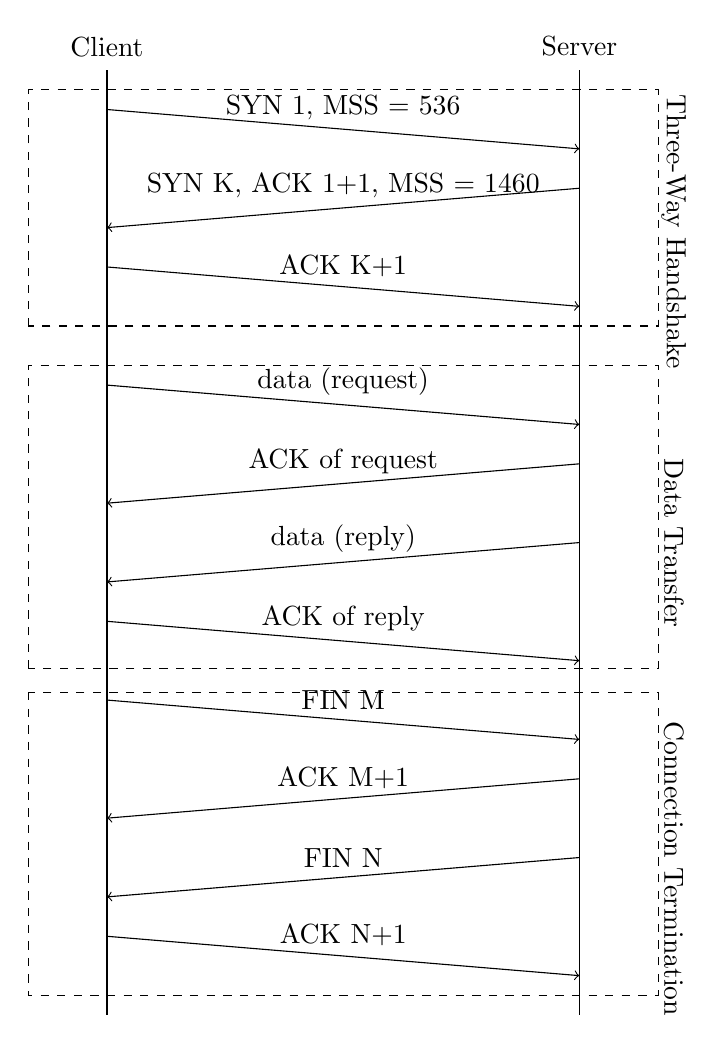
\begin{tikzpicture}
            % Drawing the vertical lines for Client and Server
            \draw (-3,0) -- (-3,-12) (3,0) -- (3,-12);
            
            % Labels for Client and Server
            \node at (-3,.3) {Client};
            \node at (3,.3) {Server};
            
            % Three-Way Handshake
            \draw[->] (-3,-0.5) -- node[midway,above] {SYN 1, MSS = 536} (3,-1);
            \draw[->] (3,-1.5) -- node[midway,above] {SYN K, ACK 1+1, MSS = 1460} (-3,-2);
            \draw[->] (-3,-2.5) -- node[midway,above] {ACK K+1} (3,-3);
            
            % Data Exchange
            \draw[->] (-3,-4) -- node[midway,above] {data (request)} (3,-4.5);
            \draw[->] (3,-5) -- node[midway,above] {ACK of request} (-3,-5.5);
            \draw[->] (3,-6) -- node[midway,above] {data (reply)} (-3,-6.5);
            \draw[->] (-3,-7) -- node[midway,above] {ACK of reply} (3,-7.5);
            
            % Connection Termination
            \draw[->] (-3,-8) -- node[midway,above] {FIN M} (3,-8.5);
            \draw[->] (3,-9) -- node[midway,above] {ACK M+1} (-3,-9.5);
            \draw[->] (3,-10) -- node[midway,above] {FIN N} (-3,-10.5);
            \draw[->] (-3,-11) -- node[midway,above] {ACK N+1} (3,-11.5);
            \draw[dashed] (-4,-3.25) rectangle (4,-0.25) 
            node[rotate=270, anchor=west, yshift=0.2cm, xshift=-2] {Three-Way Handshake};
        
            \draw[dashed] (-4,-7.6) rectangle (4,-3.75) 
            node[rotate=270, anchor=west, yshift=0.2cm, xshift=30] {Data Transfer};
        
            \draw[dashed] (-4,-7.9) rectangle (4,-11.75) 
            node[rotate=270, anchor=west, yshift=0.2cm, xshift=-102.5] {Connection Termination};
        \end{tikzpicture}
    }
}

% ─────────────────────────────────────────
\section{OSI Model}
% ─────────────────────────────────────────

{\footnotesize
\begin{tabular}{clll}
\toprule
\textbf{\#} & \textbf{Layer} & \textbf{Protocol/Unit} & \textbf{Key Function}\\
\midrule
7 & Application  & HTTP, DNS, FTP    & User-facing services\\
6 & Presentation & TLS, SSL          & Encoding, encryption\\
5 & Session      & Sockets           & Session management\\
4 & Transport    & TCP, UDP          & Segment, port, reliability\\
3 & Network      & IP, ICMP, BGP     & Packet routing\\
2 & Data Link    & Ethernet, MAC     & Frame, MAC addr, switches\\
1 & Physical     & Cables, WiFi      & Bits over medium\\
\bottomrule
\end{tabular}
}

\end{multicols}
\end{document}
